\section{Установленные улучшения и ухудшения}
\label{sec:positive_evidence}
Таблица~\ref{tab:main_effects} объединяет конкретные эффекты,
на которых основаны содержательные выводы. Для каждого эффекта
сохранены исходный контраст, направление сравнения и полная семья.
Это выбранные иллюстрации общей проверки, а не восемь независимых
репликаций; полные подсчёты приведены в приложении.

\begin{table}[htbp]\centering\footnotesize
\caption{Основные подтверждённые эффекты при fit1000 и квоте 20\%.
Interaction означает изменение разности между natural и harm8 raw.
Пары: B --- TF--IDF $\to$ frozen MiniLM; C --- TFfull $\to$ MiniLM,
кроме Ternary--Direct (TF10 $\to$ TFfull); M --- TF3 $\to$ MiniLM.
В C используется accuracy-настройка, в B и M --- MSE.
Знак соответствует первому методу минус второй.}
\label{tab:main_effects}
\begin{tabular}{lcrr}
\toprule
Сравнение / эффект & Семья & П.п. & 95\% интервал \\
\midrule
BANKING77: Direct--Weak-error, interaction & B & -4{,}87 & [-7{,}34; -2{,}40] \\
CLINC150: Direct--Weak-error, interaction & C & -2{,}00 & [-3{,}34; -0{,}66] \\
CLINC150: Hurdle--Direct, harm8 & C & 0{,}85 & [0{,}03; 1{,}66] \\
CLINC150: Hurdle--Direct, interaction & C & 0{,}87 & [0{,}06; 1{,}68] \\
CLINC150: Ternary--Direct, interaction & C & 0{,}77 & [0{,}11; 1{,}43] \\
CLINC150: Direct, IPW--raw & C & 2{,}04 & [0{,}68; 3{,}40] \\
CLINC150: Ternary--Hurdle, accuracy & M & 0{,}29 & [0{,}02; 0{,}57] \\
CLINC150: Ternary--Hurdle, macro-F1 & M & 0{,}33 & [0{,}04; 0{,}63] \\
\bottomrule
\end{tabular}

\end{table}

\subsection{BANKING77: отбор вызывает сравнительную деградацию gain-методов}
В полном сравнении BANKING77 harm8 без коррекции ухудшает
семь gain-параметризаций относительно обучаемого Weak-error
на четырёх из 21 проверенной пары: TF--IDF $\to$ frozen MiniLM,
TF--IDF $\to$ tuned MiniLM, BERT-tiny $\to$ frozen MiniLM
и TF--IDF с 3 $\to$ 10 метками на класс.
Получены 28 взаимодействий против Weak-error; ещё 28 относятся
к тем же методам против неизменного confidence.
Последний является контролем, поскольку не зависит от router-fit.

В примере TF--IDF $\to$ frozen MiniLM accuracy Direct меняется
с 91,44\% на 86,56\%, а Weak-error --- с 91,26\% на 91,25\%.
Изменение Direct--Weak-error равно \BankShiftEffect{} п.п.,
одновременный интервал $\BankShiftCI$.
Таким образом, найден именно сдвиг сравнительного качества,
а не только описательная разница двух средних.
Аналогичные взаимодействия в этой паре установлены для остальных
шести gain-методов. В семье B также подтверждены 28 ухудшений
raw-обучения относительно natural через контрасты с фиксированным
confidence и 34 положительных эффекта коррекции IPW относительно raw.

\begin{table}[htbp]\centering\small
\caption{BANKING77, TF--IDF $\to$ frozen MiniLM: средняя accuracy
в трёх составах, 20 обучений. IPW проверяется на тех же
harm8-извлечениях. Числа в таблице описательные; статистические
утверждения опираются на семью B.}
\label{tab:bank_extended}
\begin{tabular}{lrrr}
\toprule
Метод & Natural, \% & Harm8 raw, \% & Harm8 IPW, \% \\
\midrule
Weak-error & 91{,}26 & 91{,}25 & 91{,}25 \\
Direct & 91{,}44 & 86{,}56 & 91{,}49 \\
Marginal & 91{,}36 & 86{,}50 & 91{,}51 \\
Events & 91{,}45 & 86{,}50 & 91{,}52 \\
Ternary & 91{,}46 & 86{,}61 & 91{,}53 \\
Joint & 91{,}43 & 86{,}61 & 91{,}50 \\
Hurdle & 91{,}34 & 86{,}61 & 91{,}50 \\
Soft-gain & 91{,}37 & 86{,}52 & 91{,}49 \\
Confidence & 90{,}68 & 90{,}68 & 90{,}68 \\
\bottomrule
\end{tabular}

\end{table}

\subsection{CLINC150: воспроизведение сравнительной деградации}
На CLINC150 TFfull $\to$ MiniLM при MSE-настройке Direct меняется
с 94,68\% на 92,78\%, Weak-error --- с 94,71\% на 94,74\%.
При настройке по квотной accuracy Direct меняется с 94,68\%
на 92,69\%, Weak-error --- с 94,70\% на 94,71\%.
Для второго варианта изменение Direct--Weak-error равно
\ClincShiftEffect{} п.п., интервал $\ClincShiftCI$,
скорректированное $p=\ClincShiftP$.
Следовательно, обнаруженный тип сравнительной деградации
воспроизводится в новой панели и сохраняется при эксплуатационном
критерии настройки. Это проверка конкретного явления на втором
датасете, а не усреднение независимых эффектов по всем парам.

\begin{table}[htbp]\centering\small
\caption{CLINC150, TFfull $\to$ MiniLM: средняя accuracy,
accuracy-настройка, fit1000, квота20\%, 20 обучений.}
\label{tab:clinc_extended}
\begin{tabular}{lrrr}
\toprule
Метод & Natural, \% & Harm8 raw, \% & Harm8 IPW, \% \\
\midrule
Weak-error & 94{,}70 & 94{,}71 & 94{,}71 \\
Direct & 94{,}68 & 92{,}69 & 94{,}74 \\
Marginal & 94{,}69 & 92{,}95 & 94{,}72 \\
Events & 94{,}68 & 92{,}88 & 94{,}71 \\
Ternary & 94{,}69 & 92{,}92 & 94{,}71 \\
Joint & 94{,}68 & 92{,}94 & 94{,}71 \\
Hurdle & 94{,}66 & 93{,}54 & 94{,}73 \\
Soft-gain & 94{,}65 & 92{,}72 & 94{,}71 \\
Confidence & 94{,}47 & 94{,}47 & 94{,}47 \\
\bottomrule
\end{tabular}

\end{table}

\subsection{Внутри gain-семейства: Hurdle теряет меньше, чем Direct}
\textbf{В harm8 raw Hurdle превосходит Direct на
\HurdleSimpleEffect{} п.п.} Для TFfull $\to$ MiniLM
его accuracy составляет 93,54\% против 92,69\% у Direct.
Простой одновременный интервал разности Hurdle--Direct равен
$\HurdleSimpleCI$, скорректированное $p=\HurdleSimpleP$.
На natural средние составляют 94,66\% и 94,68\% соответственно.
Отдельный тест взаимодействия даёт
$\Delta_{\mathrm{Hurdle,Direct}}=\HurdleShiftEffect$ п.п.,
интервал $\HurdleShiftCI$, $p=\HurdleShiftP$.
Тем самым установлены одновременно выигрыш Hurdle в данном
harm-режиме и изменение относительного качества между составами.
Поскольку оба метода теряют относительно natural, интерпретация
этого результата --- \emph{меньшая деградация Hurdle}.

Всего при accuracy-настройке подтверждены восемь из 126
gain-only взаимодействий на трёх парах: TF3 $\to$ TF10,
TF10 $\to$ TFfull и TFfull $\to$ MiniLM.
Все восемь сохраняются при увеличении числа bootstrap-повторов
с 2\,000 до 10\,000; полный список дан в приложении.
Например, для TF10 $\to$ TFfull изменение Ternary--Direct
равно \TernaryShiftEffect{} п.п. с интервалом $\TernaryShiftCI$.
Следовательно, неодинаковая чувствительность наблюдается
не только между gain-целью и прогнозом ошибки первого эксперта,
но и между реализованными параметризациями одной идеальной полезности.

\begin{figure}[htbp]\centering
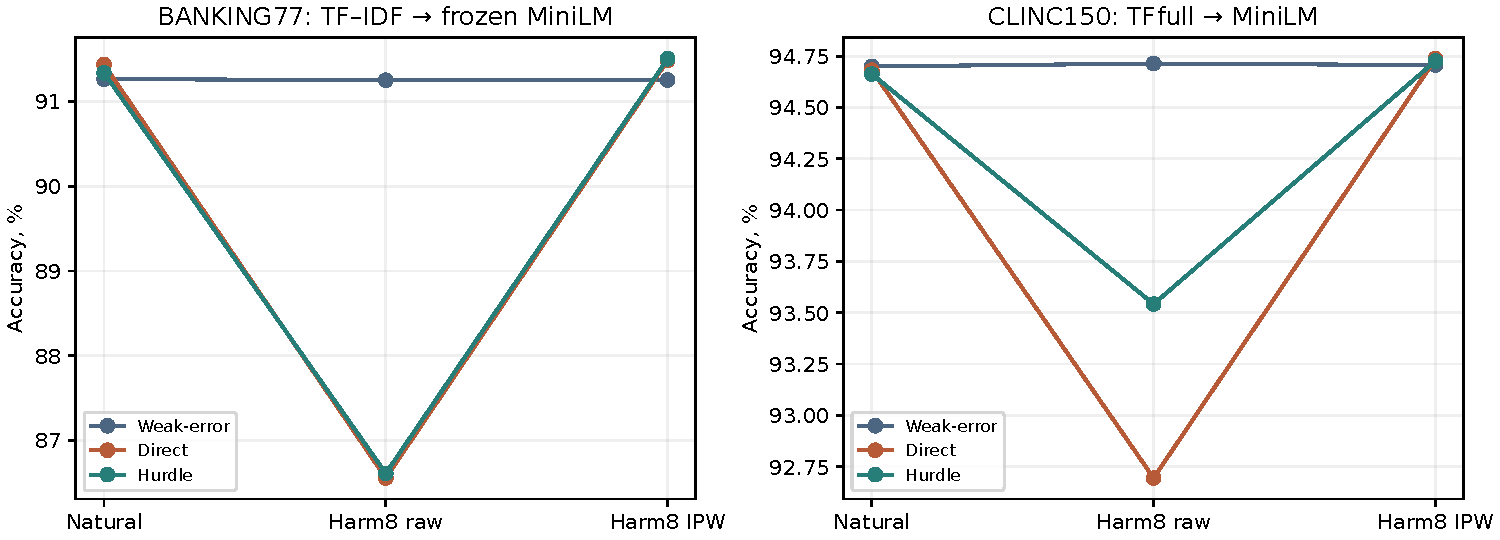
\includegraphics[width=\linewidth]{additions/figures/composition_effects.pdf}
\caption{Изменение средней accuracy при natural, harm8 raw и harm8 IPW.
Слева --- BANKING77, MSE-настройка; справа --- CLINC150,
accuracy-настройка. Линии показывают средние, без доверительных полос;
неопределённость соответствующих контрастов приведена в
таблице~\ref{tab:main_effects}.}
\label{fig:composition_extended}
\end{figure}

\subsection{Коррекция даёт измеримый прирост над raw-обучением}
В той же паре CLINC150 IPW повышает accuracy Direct с 92,69\%
до 94,74\%: эффект равен \CorrectionEffect{} п.п., интервал
$\CorrectionCI$, $p=\CorrectionP$.
Raw и IPW используют одинаковые fit-строки, признаки,
стандартизацию и сетку регуляризации; меняются веса обучающей потери,
а регуляризация выбирается по одному и тому же правилу.
Это контролируемое улучшение полного способа обучения с коррекцией.

Содержательный смысл состоит в восстановлении качества,
утраченного при известном смещении: natural-среднее Direct равно
94,68\%. Сравнение не следует представлять как выигрыш нового
роутера над естественным обучением. Возвращение средних к исходному
уровню и установленный IPW--raw эффект согласуются с изменением
условной цели в формуле~\eqref{eq:selection_shift}.
Поэтому при выборе по отобранной разметке нужны оба контроля:
простой обучаемый Weak-error и корректно взвешенные gain-кандидаты.
